% Asset ID: FA22GeneratingFunctionsTikZ-003
% Unit: FA22 – Further A2 2 Applied Mathematics
% Topic code: FA22-GENFUNC
% Topic ID: FA22GeneratingFunctions
% Related lesson: FA22_generating_functions_lesson.md
% Source status: Optional enrichment, not confirmed CCEA core
\documentclass[tikz,border=8pt]{standalone}
\usepackage{amsmath}\usepackage{xcolor}\usetikzlibrary{arrows.meta,positioning,calc}
\definecolor{Canvas}{HTML}{FAF9F6}\definecolor{Ivory}{HTML}{FFFFF0}\definecolor{Line}{HTML}{E5E5EA}\definecolor{Gold}{HTML}{C5A059}\definecolor{SoftPink}{HTML}{FBEFEF}\definecolor{Text}{HTML}{2C2C2E}
\begin{document}
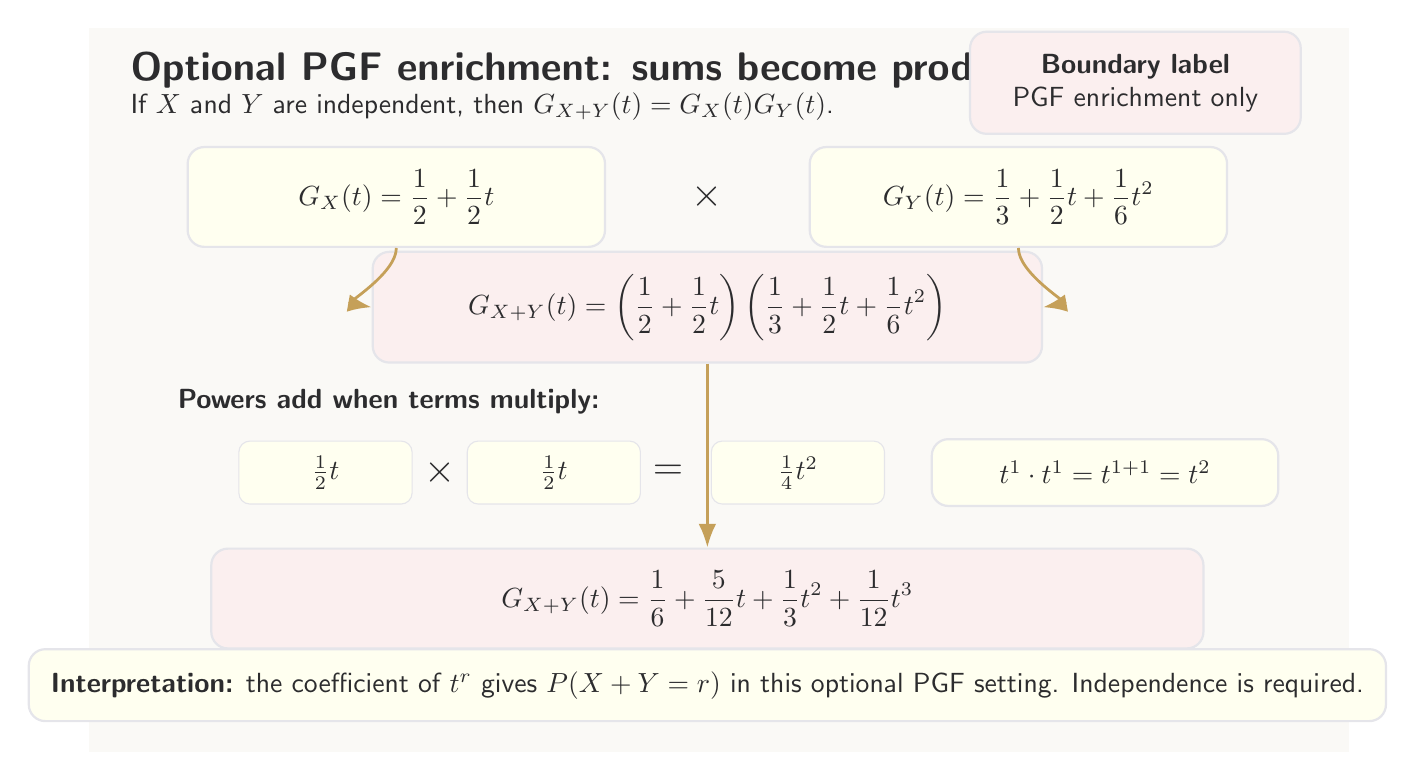
\begin{tikzpicture}[font=\sffamily,text=Text,box/.style={draw=Line,fill=Ivory,rounded corners=6pt,line width=0.8pt,align=center,inner sep=8pt},accentbox/.style={draw=Line,fill=SoftPink,rounded corners=6pt,line width=0.8pt,align=center,inner sep=8pt},arrow/.style={-{Latex[length=3mm]},line width=1pt,draw=Gold},tinyterm/.style={draw=Line,fill=Ivory,rounded corners=4pt,minimum width=2.2cm,minimum height=0.8cm,align=center}]
\fill[Canvas] (-0.8,-3.2) rectangle (15.2,6.0);
\node[anchor=west,font=\sffamily\bfseries\Large] at (-0.4,5.45){Optional PGF enrichment: sums become products};
\node[anchor=west,font=\sffamily\normalsize] at (-0.4,5.0){If \(X\) and \(Y\) are independent, then \(G_{X+Y}(t)=G_X(t)G_Y(t)\).};
\node[accentbox,anchor=east,minimum width=4.2cm] at (14.6,5.3){\textbf{Boundary label}\\PGF enrichment only};
\node[box,minimum width=5.3cm] (GX) at (3.1,3.85){\(\displaystyle G_X(t)=\frac12+\frac12t\)};
\node[box,minimum width=5.3cm] (GY) at (11.0,3.85){\(\displaystyle G_Y(t)=\frac13+\frac12t+\frac16t^2\)};
\node[font=\sffamily\bfseries\Large] at (7.05,3.85){\(\times\)};
\node[accentbox,minimum width=8.5cm] (product) at (7.05,2.45){\(\displaystyle G_{X+Y}(t)=\left(\frac12+\frac12t\right)\left(\frac13+\frac12t+\frac16t^2\right)\)};
\draw[arrow] (GX.south) to[out=-90,in=170] (product.west);\draw[arrow] (GY.south) to[out=-90,in=10] (product.east);
\node[anchor=west,font=\sffamily\bfseries] at (0.2,1.25){Powers add when terms multiply:};
\node[tinyterm] at (2.2,0.35){\(\frac12t\)};\node[font=\Large] at (3.65,0.35){\(\times\)};\node[tinyterm] at (5.1,0.35){\(\frac12t\)};\node[font=\Large] at (6.55,0.35){\(=\)};\node[tinyterm] at (8.2,0.35){\(\frac14t^2\)};\node[box,minimum width=4.4cm] at (12.1,0.35){\(t^1\cdot t^1=t^{1+1}=t^2\)};
\node[accentbox,minimum width=12.6cm] (result) at (7.05,-1.25){\(\displaystyle G_{X+Y}(t)=\frac16+\frac{5}{12}t+\frac13t^2+\frac{1}{12}t^3\)};
\draw[arrow] (product.south) -- (result.north);
\node[box,minimum width=12.6cm] at (7.05,-2.35){\textbf{Interpretation:} the coefficient of \(t^r\) gives \(P(X+Y=r)\) in this optional PGF setting. Independence is required.};
\end{tikzpicture}
\end{document}
